\documentclass{article}
\usepackage{graphicx} % Required for inserting images
\graphicspath{{Images/}}
\usepackage[utf8]{inputenc}
\usepackage{multicol}
\usepackage{amsthm}
\usepackage{amsmath}
\usepackage{xcolor}
\usepackage{subfigure}


\newtheorem{definition}{Definition}[section]
\newtheorem{remark}{Remarque}[section]
\newtheorem{theorem}{Théorème}

\title{Algèbre Linéaire}
\author{Laura Paraboschi / Simon Lefort }
\date{BA1 - IN}

\begin{document}

\maketitle

\section{Equations linéaires}
\begin{definition}
    Une équation linéaire est de la forme :
    \[ a_1x_1 + a_2x_2 + ... + a_nx_n = b \]
    Pour des nombres \( a_1, \ a_2, \ ..., \ a_n \ \)et b indépendants des variables
\end{definition}
\begin{multicols}{2}
    \begin{figure}[h]
        \centering
        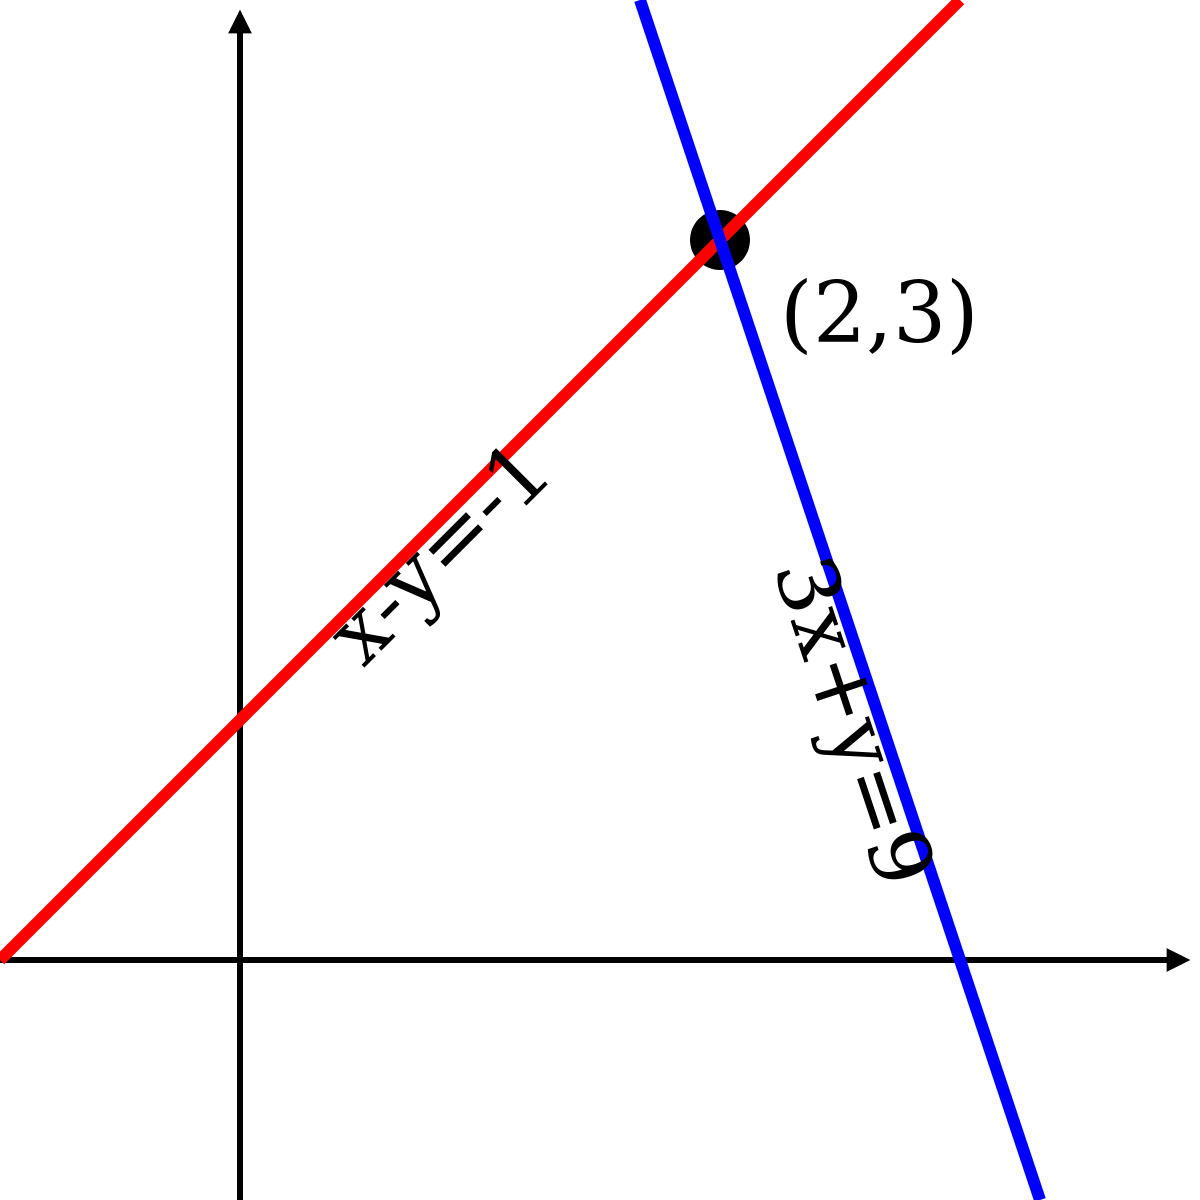
\includegraphics[width=4cm]{Images/1200px-Intersecting_Lines.svg.png}
        \caption{à 2 inconnues}
        \label{fig:Graphe 2 inconnues}
    \end{figure}
\columnbreak
    \begin{figure}[h]
        \centering
        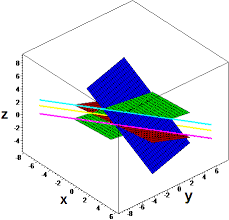
\includegraphics[width=4cm]{Images/Plans.png}
        \caption{à 3 inconnues}
        \label{fig:Graphe 2 inconnues}
    \end{figure}
\end{multicols}
\end{document}
